\documentclass[../TFG_Report.tex]{subfiles}
 
\begin{document}
	
As the aim of the project is to design a new product, a good knowledge of the state of the art is necessary to have a starting point. In this section the current framework of small wind turbines will be described. 
	
\subsection{History and impact of small wind turbines}

The first steps in the development of small and micro wind turbines took place during the thirties, with the objective of charging batteries in remote households. Manufacturers like Jacobs \cite{Jacobs} or Parris-Dunn \cite{Parris} produced this type of wind turbines in the United States. In the late forties, with the arrival of the electrical grid to the rural areas, this industry practically disappeared. It remained in hibernation until the seventies, when the petrol crisis created the need for alternative energy sources. Tha attention came back to the small wind turbine energy, not only in the United States but also in Europe, where, for example, the Bornay brothers started their company in Spain \cite{Bornay}. \\

During the eighties this technology started to evolve, as the manufacturers began to abandon the DC dynamo generators and incorporated synchronous generators with permanent magnets (AC). In order to obtain a DC current for charging batteries, rectifiers were needed. Over time these rectifiers were connected to inverters to be able to connect the wind turbines to the grid. Induction generators began to be used as well in order to connect them directly to the grid, but it was a difficult solution to implement in isolated applications due to the generator's need to be excited from outside. The need for a gearbox also difficulted its success.The size and power produced started growing gradually, and before the ending of the eighties 50kW was considered a small wind turbine, with diameters of more than 15m. \cite{Sanz} The current regulations (IEC 61400-2 \cite{IEC}) establish that the limit of a small wind turbine is given by a swept area smaller than 200m$^2$. \\

The small wind turbines technology has been evolving from the isolated applications to he modern grid-connected installations, and has even entered into the residential and urban outline. These last applications have caused the increased use of vertical axis solutions. The most well known developments are the Savonius and Darrenius wind turbines, but also the Gorlov design and some combined schemes are being used. \cite{Sanz}  \\

Regarding the impact of the small wind energy, the last World Wind Energy Association (WWEA) report indicates, from 2014 data, that there were 945,000 small wind turbines installed all over the world, producing almost 850MW. China and USA are clearly leading this market, and the biggest market in Europe is in the UK. Unfortunately, developing countries have an anecdotal presence, even though this was a technology initially developed with the objective of electrifying isolated regions, and the enormous wind power potential (especially in the eastern highlands of Africa) . All of this can be seen in the following figure: 

\begin{figure}[h!]
	\centering
	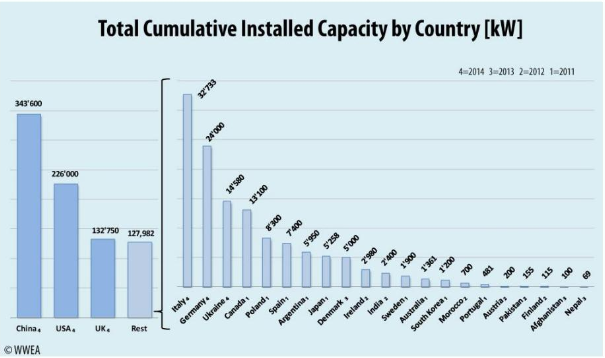
\includegraphics[width=0.85\linewidth]{Images/Total_cumulative_instlled_capacity}
	\caption[Total cumulative installed capacity of SWT by country]{Total cumulative installed capacity of SWT by country. \\
		Obtained from WWEA 2016 report.}
	\label{fig:totalcumulativeinstlledcapacity}
\end{figure}

The forecast for new installations in this report predicted a big growth in the annual installed capacity. Unfortunately there is no data available or a newer WWEA report to check the last tendency of the market. 

\begin{figure}[h!]
	\centering
	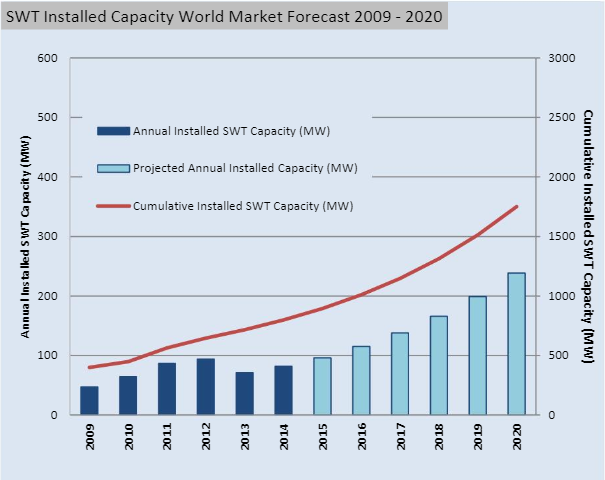
\includegraphics[width=0.85\linewidth]{Images/SWT_Installed_capacity_forecast}
	\caption[SWT installed capacity forecast]{Small Wind Turbines installed capacity forecast. \\
		Obtained from WWEA 2016 report.}
	\label{fig:swtinstalledcapacityforecast}
\end{figure}

\FloatBarrier

Analyzing the perspectives in Spain, the last Renewal Energy Plan (PER) established the objective of reaching 300MW installed in 2020, predicting more than 50MW of new installations every year on from 2020. \cite{PER} \\

The investment in this kind of wind turbines is usually made by private individuals or small communities in order to partially or totally fulfill their demand for electricity or heating. However, a large portion of the buyers is disappointed by the actual energy obtained from these wind turbines. The main reason for this is the promotion of inaccurate and overstated information of the power output by manufacturers or installers. The satisfaction and reviews of this kind of products can spread very fast, and this type of feedback is reducing the confidence of this sort of economic investing, consequently slowing down this sector's growth. \cite{DesignControl}





%%POSAR ALGO MÉS DE TENDENCIES i coses x promocionar la mini eolica 



 



\subsection{Advantages and disadvantages}

The generation of electricity through small wind turbines has some particular advantages and disadvantages in comparison to larger wind turbines or other sources of renewable energy. In this section these particular characteristics will be enumerated. \cite{Sanz} \cite{Apunts}

\subsubsection{Advantages}

\begin{enumerate}
	\item \textbf{Renewable energy}: It is virtually inexhaustible and does not produce air emissions nor pollution. 
	
	\item It can \textbf{coexist} with other installations and land uses (for example agriculture).
	
	\item Easy and fast \textbf{installation}: the study made in section \ref{State_market} shows that a strong point of commercial SWTs is the possibility of an easy installation, which facilitates direct sale to the final user.
	 
	\item Suitable for \textbf{isolated areas} due to the possibility of battery charging applications and integration with other types of generation. It allows the possibility to achieve electric energy independence. 
	
	\item Energy is generated close to the consumption points, which reduces the \textbf{transportation losses}. It also does not require additional big installations for transportation and evacuation of electricity.
	
	\item \textbf{Reduced maintenance and operation costs}, and high reliability. 
	  
	\item Less \textbf{environmental} and \textbf{visual} \textbf{impact}. 
	
	\item Can be generally optimized for \textbf{moderated wind speeds}, which eliminates the need for complex viability studies and allows a better production in average installation sites. 
	
\end{enumerate}


\subsubsection{Disadvantages}

\begin{enumerate}
	\item The wind is intermittent, uncontrollable and relatively unpredictable, so \textbf{other sources of energy are required} to ensure enough electricity production.
	
	\item The \textbf{visual impact} can still be a drawback. 
	
	\item The \textbf{noise} is important in residential areas. 
	
	\item \textbf{Flickering}: visual phenomena produced by the periodic projection of the blades shadow. 
	
	\item \textbf{Lack of complex active control systems} due to price limitations. SWTs are generally simpler than large wind turbines. 
	
\end{enumerate}




	
\subsection{Design solutions}

The design of any wind turbine in general has multiple options and solutions. In this and the following section these alternatives will be analyzed, first with an explanation of each solution and then with its presence and importance in the market. The main different approaches for small wind turbines will be explained below: the axis orientation (horizontal axis wind turbines (HAWTs) and vertical axis wind turbines (VAWTs)), the rotor position in relation to the tower (upwind and downwind), the addition of a duct (diffusor augmented wind turbines DAWTs), the number of blades and the power control.   \\

\subsubsection{Axis orientation}

The major classification of wind turbines is commonly made from the position of the rotor axis of revolution: HAWTs and VAWTs. The most used solution is the horizontal design. As the small wind energy world usually follows the developments of the large wind turbines industry, close to 75\% of SWTs are HAWTs. However, VAWTs have some advantages: they are conceptually simpler (since they do not require a yawing mechanism), there are some structural and maintenance benefits (the generator and the gearbox are placed close to the ground), and they need a lower cut-in wind speed. VAWTs can be based on drag (Savonius) or on lift (Darrenius), which is a much more efficient approach. A lot a of research is being done in the latter, as the aerodynamics are much more complex than HAWTs, and the overall performance is growing. VAWTs have been gaining presence in the last years, especially in urban environments. \cite{Handbook} \cite{DesignControl}

\subsubsection{Rotor position}

The wind turbines can also be divided by the position of the rotor in relation to the tower. The most common solution is using upwind wind turbines, situating the blades (relatively to the wind) in front of the tower (windward). The other alternative is called downwind, where the rotor is located on the back side of the turbine. \\

\begin{figure}[h!]
	\centering
	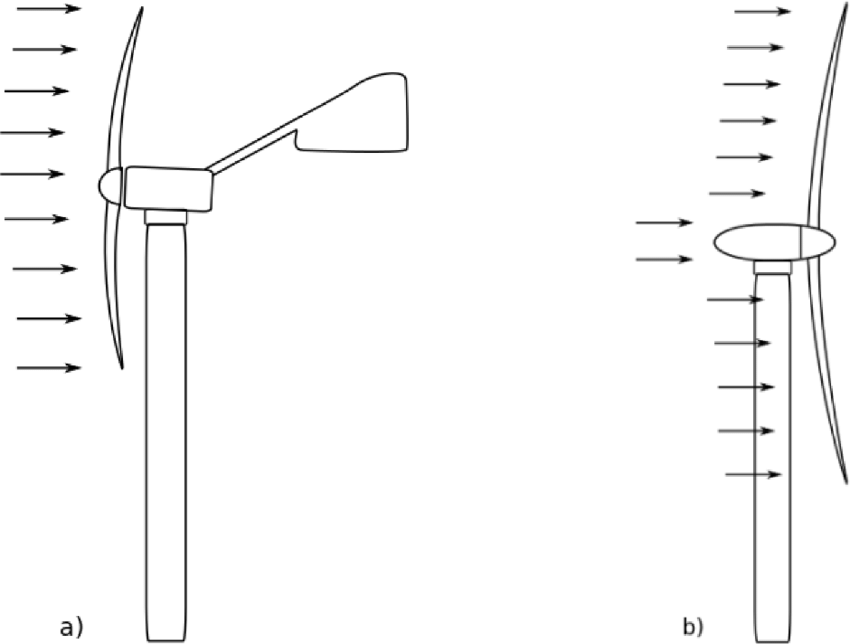
\includegraphics[width=0.4\linewidth]{Images/Upwind-a-and-downwind-b-wind-turbines}
	\caption[Upwind and downwind wind turbines]{Upwind (a) and downwind (b) wind turbines. \\ Extracted from \cite{DesignControl}.}
	\label{fig:upwind-a-and-downwind-b-wind-turbines}
\end{figure}


The upwind wind turbines are characterized by a higher efficiency, as the impact of the tower and the nacelle to the incoming wind is much smaller in this configuration. However, there is risk of collision between the rotor and the tower, so the blades are required to have a higher stiffness or either be placed with some angle or distance. Another drawback of this design is the need of a yaw system in order to keep the rotor facing the wind, as the natural trend of the rotor is to move to the downwind position. In the SWTs this is usually accomplished using a tail vane.   \\

These special requirements of the upwind wind turbines are precisely one of the principal advantages of the downwind design: they are simpler. The lack of these needs is also beneficial in regard to the structural dynamics and weight of the wind turbine. The main disadvantage is the influence of the tower and the nacelle to the incoming wind profile, which leads to fluctuations of momentum in the blades. The fatigue damage and the resonance risk are a real danger to take into account. The noise generated is higher, as the turbulence produced by the tower will impact the blades. \cite{DesignControl}

\subsubsection{Diffusor augmented wind turbines}

An innovative design for HAWTs is the usage of a circular duct that encapsulates the rotor. These wind turbines are called DAWT, compact wind acceleration turbine (CWAT) or wind lens. The objective of this solution is to accelerate and uniformize the incoming flow through the rotor. Some studies have shown in wind tunnel test the benefits of this system \cite{DAWT}, but little results are obtained in real outside conditions. The added mass due to the diffusor puts more stress in the tower and makes the operation of the yaw system more difficult. However, it is not strange to see this kind of system in boat's SWTs. \cite{DesignControl}


\subsubsection{Number of blades}

The selection of the number of blades (only referring to HAWTs) is a compromise between different aspects. The effects of varying the number of blades can be analyzed from both an aerodynamic and a dynamic perspective. \\

From the aerodynamic point of view, the performance (power coefficient) increases with the number of blades, but this effect has less importance from 3 blades on. The optimal rotational speed, on the other hand, decreases with the number of blades, and this is important to take into account because the aerodynamic noise produced (the most predominant)  scales with the fifth power of the blade tip speed. \\

From the dynamic point of view, the main goal is to reduce the rotating mass in order to diminish the loads that the structure will have to support. The weight of each blade is important. \\

\begin{figure}[h!]
	\centering
	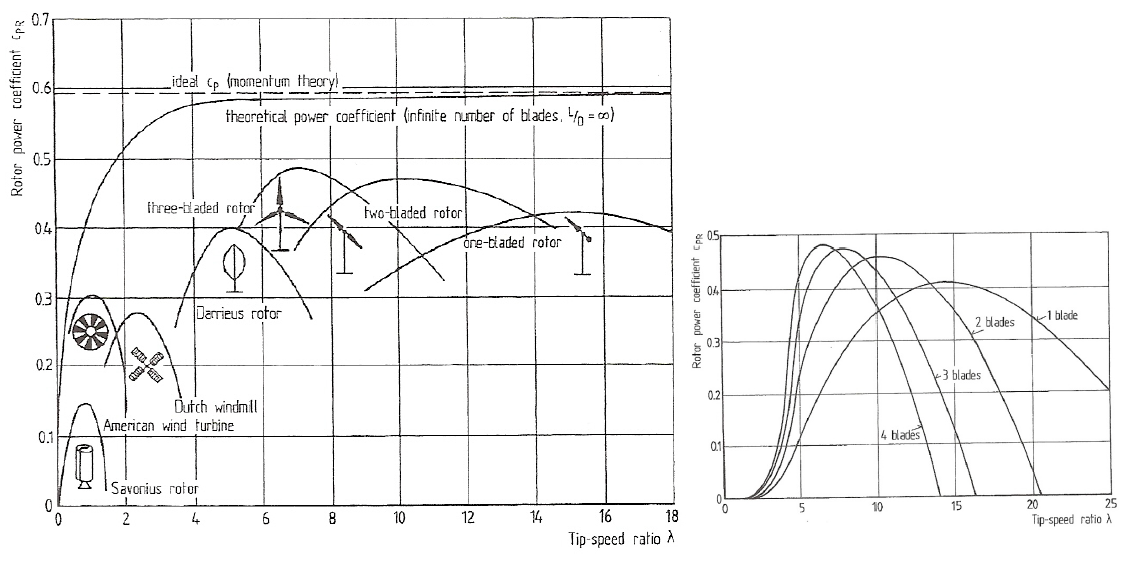
\includegraphics[width=1\linewidth]{Images/Cp_number_blades}
	\caption[Power coefficient as a function of the number of blades and wind turbine type]{Power coefficient as a function of the number of blades and wind turbine type. \\ Extracted from \cite{Apunts}.}
	\label{fig:cpnumberblades}
\end{figure}

The dominant solution for multi-megawatts wind turbines is the three-bladed rotor. More variety is observed in the world of SWTs, but the most used design is composed of three blades as well. The main advantage of this design is a higher stability: the power output oscillates less during a turn, the gravitational and gyroscopic forces are better balanced (reduction of vibration problems), and a smoother operation is achieved. The noise and the visual impact are also reduced. However, they are heavier and more complex in general than two or one-bladed rotors, and the installation and control system are more complicated. \cite{Apunts}

\subsubsection{Power control}

Once the generator reaches nominal power, a control system is required in order to maintain this value. This control system is also necessary to protect the wind turbine in case of stronger winds. If the wind speed exceeds the one required to reach nominal power, this system will waste part of the excess energy in order to avoid damaging the wind turbine. This is achieved, typically, by either an active pitch control or a passive stall control. \\

In a passive stall control system, the blades are bolted onto the hub at a fixed angle. As the actual angle of attack of the blades increases with the wind speed, the fixed pitch and twist of the blade can be designed in order to get the blades to stall at a desired point. If the rotor stalls, the torque and power generated will diminish. This solution avoids the need of a complex variable pitch system, but higher loads will be experienced, and an aerodynamic brake will be required. \\

On a pitch controlled wind turbine, there is an electronic controller that receives the generator's power output. If this magnitude becomes excessively high, the controller varies the pitch of the blades. The effective angle of attack is reduced, and the torque and power produced by the blades drop. \cite{Dromstorre}



\subsection{State of the market} \label{State_market}

The table \ref{state_of_market} indicates a sample of the small wind turbines that can be commonly found in the market nowadays. Some interesting conclusions can be extracted from it:

\begin{enumerate}
	\item The dominant design is the \textbf{horizontal axis wind turbine}, as seen in the preceding section. 
	\item All of them use \textbf{direct drive} configuration (lack of gearbox).
	\item All mention a \textbf{low start torque} resulting in a low start wind speed (between 2 m/s and 4 m/s). However, it has been seen that the power output at these wind speeds is also very low. The objective of this feature could be an automatic starting procedure.
	\item The usage of \textbf{UV protection coatings} on the blades.
	\item The \textbf{installability} and the \textbf{low noise production} are essential characteristics from a commercial point of view. 
	\item Almost all of them are configured for \textbf{battery charging applications}, and some of them have one version for grid connexion and another one for battery charging at 24/48 V. 
	\item Most of them require a \textbf{tower} of at least 10 m height to reach nominal power (by manufacturer indication). However, almost none of them include it. Some brands offer the tower separately from the wind turbine, which is sold at almost the same prize as the wind turbine itself.
	
\end{enumerate}





\begin{landscape}
\begin{table}
	\centering
	\rowcolors{2}{}{lightgray}
	\caption{State of the market of small wind turbines.}
	\label{state_of_market}
{\small
\begin{tabular}{|>{\centering}m{2.5cm}|>{\centering}m{2cm}|>{\centering}m{1.3cm}|>{\centering}m{1.5cm}|>{\centering}m{1cm}|>{\centering}m{1.5cm}|>{\centering}m{1.5cm}|>{\centering}m{1.5cm}|>{\centering}m{2cm}|>{\centering}m{2cm}|c|}
	\hline
	Manufacturer and Model 
	              & Architecture                    & Number of blades & Rotor diameter {[}m{]} & RPM     & Nominal wind speed {[}m/s{]} & Nominal power {[}W{]} & Material                      & Control system                                 & Generator                                 & Weight {[}kg{]} \\ \hline \hline
	Bornay 13    \cite{Bornay}                & HAWT, Upwind  & 2                & 2.86                   & @600    & 12                           & 1500                  & Carbon or glass fiber            & Electronic regulator and pasive by inclination & Trifasic with permanent Neodymium magnets & 41              \\ \hline
	Bornay Bee 800      \cite{Bornay}         & HAWT, Upwind   & 5                & 1.75                   & @500    & 12                           & 800                   & Injected nylon                & Electronic controller                          & Trifasic with permanent Neodymium magnets & 29              \\ \hline
	Enair E30 PRO     \cite{Enair}          & HAWT, Upwind, self regulating   & 3                & 3.80                   & 250     & 11                           & 1900                  & Glass fiber                   & Passive pitch control with two action speeds   & Neodymium permanent magets (30 poles)     & 125             \\ \hline
	SD Wind Energy SD3    \cite{SD_Wind_E}               & HAWT, Downwind, self regulating & 3                & 3.90                   & Màx 300 & -                            & 3000                 & Glass Thermoplastic Composite & Passive                                        & Brushless permanent magnets               & -               \\ \hline
	Smarttwister ST-1000    \cite{Smarttwister}           & VAWT, Helicoidal blade          & 1                & 0.34 (1.38m height)    & 525     & 7.6                          & 1000                  & Technic nylon                 & Electronic controller                          & Neodymium permanent magnets               & 34              \\ \hline
	Aeolos V 300W     \cite{Aeolos}           & VAWT                            & 3                & 1.20 (1.60m height)    & 300     & 10                           & 300                   & Aluminum alloy                & -                                              & Permanent magnets                         & 10              \\ \hline
	Bergey Excel 1     \cite{Bergey}          & HAWT, Upwind, self regulating                    & 3                & 2.50                   & -       & 11                           & 1000                  & Glass fieber                  & Furling against high wind speeds               & Neodymium permanent magets                & 34              \\ \hline
	AutoMaxx DB-400   \cite{AutoMaxx}             & HAWT, Upwind                    & 3                & 1.22                   & -       & 13                           & 400                   & Nylon and glass fiber         & Electronic controller                          & Brushless permanent magnets               & 10              \\ \hline
	MarsRock 400W Economy Windmill \cite{MarsRock}   & HAWT, Upwind                    & 3                & 1.40                   & 400     & 13                           & 400                   & Nylon and glass fiber         & Electronic controller                          & Trifasic with permanent magnets           & 10              \\ \hline
\end{tabular}
}
\end{table}




\end{landscape}




\end{document}